\documentclass[11pt,letterpaper]{article}

% ---------- Idioma y tipografia ----------
\usepackage{fontspec}
\usepackage{polyglossia}
\setdefaultlanguage{spanish}
\setmainfont{Latin Modern Roman}
\gappto\captionsspanish{\renewcommand{\tablename}{Tabla}\renewcommand{\contentsname}{Contenido}}
\setsansfont{Latin Modern Sans}
\setmonofont{Latin Modern Mono}

\usepackage[margin=2.5cm,headheight=14pt]{geometry}
\usepackage{amsmath,amssymb}
\usepackage{siunitx}
\sisetup{output-decimal-marker={,},group-separator={.},detect-all}
\usepackage{booktabs,longtable,tabularx,array,multirow,colortbl}
\usepackage[table]{xcolor}
\usepackage{graphicx,float}
\usepackage{caption}
\captionsetup{font=small,labelfont=bf,labelsep=period}
\usepackage{enumitem}
\setlist{itemsep=2pt,topsep=4pt}
\usepackage{fancyhdr}
\usepackage{titlesec}
\usepackage{microtype}
\usepackage{tocloft}
\setlength{\cftbeforesecskip}{3pt}
\renewcommand{\cftsecfont}{\bfseries\color{azuluni}}
\renewcommand{\cfttoctitlefont}{\large\bfseries\color{azuluni}}
\setlength{\cftbeforetoctitleskip}{0pt}
\setlength{\cftaftertoctitleskip}{6pt}
\usepackage{tikz}
\usetikzlibrary{shapes.geometric,arrows.meta,positioning,fit,backgrounds}
\usepackage{pgfplots}
\pgfplotsset{compat=1.18}
\usepackage[colorlinks=true,linkcolor=azuluni,citecolor=azuluni,urlcolor=azuluni]{hyperref}
\usepackage{tcolorbox}

\definecolor{azuluni}{RGB}{0,51,102}
\definecolor{grisfila}{RGB}{242,244,247}
\definecolor{resalte}{RGB}{255,244,214}

\titleformat{\section}{\large\bfseries\color{azuluni}}{\thesection.}{0.6em}{}
\titleformat{\subsection}{\normalsize\bfseries}{\thesubsection.}{0.6em}{}

\pagestyle{fancy}
\fancyhf{}
\fancyhead[L]{\small Comunicaciones Celulares}
\fancyhead[R]{\small Red LTE, Parte 1: Cobertura}
\fancyfoot[L]{\small J. A. Betancourt Saco (200144723)}
\fancyfoot[R]{\small \thepage}
\renewcommand{\headrulewidth}{0.4pt}

\newcommand{\dB}{\,\mathrm{dB}}
\newcommand{\dBm}{\,\mathrm{dBm}}
\newcolumntype{L}{>{\raggedright\arraybackslash}X}
\newcolumntype{C}{>{\centering\arraybackslash}X}

\newtcolorbox{nota}[1]{colback=resalte,colframe=azuluni!70,boxrule=0.5pt,arc=1pt,
  left=6pt,right=6pt,top=4pt,bottom=4pt,title={#1},fonttitle=\bfseries\small,coltitle=white,colbacktitle=azuluni!85}

\hypersetup{pdftitle={Diseño de una red celular LTE. Parte 1: Cobertura},
            pdfauthor={Juan Andrés Betancourt Saco}}

\begin{document}

% ================= PORTADA =================
\begin{titlepage}
\centering
\vspace*{1.2cm}
{\large\scshape Universidad del Norte\par}
{\normalsize Departamento de Ingeniería Eléctrica y Electrónica\par}
\vspace{2.2cm}
{\normalsize\scshape Comunicaciones Celulares\par}
\vspace{0.6cm}
\rule{\textwidth}{0.8pt}\par\vspace{0.4cm}
{\LARGE\bfseries Diseño de una red celular LTE\par}
\vspace{0.25cm}
{\Large Parte 1: Dimensionamiento de cobertura\par}
\vspace{0.4cm}
\rule{\textwidth}{0.8pt}\par
\vspace{0.8cm}
{\large Localidades de San Cristóbal y Usme, Bogotá D.C.\par}
\vspace{2.6cm}
{\large Juan Andrés Betancourt Saco\par}
{\normalsize Código 200144723\par}
\vfill
{\normalsize Barranquilla, 16 de octubre de 2026\par}
\vspace*{0.8cm}
\end{titlepage}

% ================= RESUMEN =================
\thispagestyle{fancy}
\begin{abstract}
\noindent Se dimensiona por cobertura una red LTE FDD de \SI{20}{MHz} en la banda 2 (PCS \SI{1900}{MHz}) del operador Claro para el área urbana de las localidades de San Cristóbal y Usme, que suma \SI{47.68}{km^2} en 12 UPZ. Con la estación típica tipo 3 (antena a \SI{30}{m}, MCS 12) y el modelo de propagación COST-231 Hata, la máxima pérdida de trayecto permitida (MAPL) es de \SI{131.96}{dB} en el enlace descendente y de \SI{128.12}{dB} en el ascendente. Los radios de celda resultantes son \SI{0.693}{km} y \SI{0.561}{km}; el enlace ascendente limita y fija el radio efectivo en \SI{0.561}{km}. Cada eNB de tres sectores cubre \SI{0.613}{km^2}, por lo que se requieren \textbf{78 eNB}. Las estaciones se distribuyen en una malla hexagonal con distancia entre sitios de \SI{842}{m}, que cubre el \SI{97.4}{\percent} del área con el radio de diseño. Se entrega el archivo KML con la ubicación de cada eNB y la huella de sus sectores, y se seleccionan equipos Ericsson y antenas Andrew (CommScope) disponibles en el mercado.
\end{abstract}

\begin{table}[H]
\centering
\caption{Resumen de resultados del dimensionamiento.}
\label{tab:resumen}
\rowcolors{2}{grisfila}{white}
\begin{tabular}{@{}ll@{}}
\toprule
\textbf{Resultado} & \textbf{Valor} \\
\midrule
Operador y banda & Claro Colombia, LTE banda 2 (FDD), \SI{20}{MHz} \\
Estación típica escogida & Tipo 3 ($h_t=\SI{30}{m}$, SF $=\SI{8}{dB}$, PL $=\SI{9}{dB}$, MCS 12) \\
MAPL DL / UL & \SI{131.96}{dB} / \SI{128.12}{dB} \\
Radio de celda DL / UL & \SI{0.693}{km} / \SI{0.561}{km} \\
Radio efectivo & \SI{0.561}{km} (limitado por UL) \\
Área por eNB (3 sectores) & \SI{0.613}{km^2} \\
Área de diseño $A_D$ & \SI{47.68}{km^2} (12 UPZ) \\
Número de eNB & $77{,}7 \rightarrow \mathbf{78}$ \\
Distancia entre sitios (ISD) & \SI{0.842}{km} \\
\bottomrule
\end{tabular}
\end{table}

\vspace{0.3cm}
{\small\tableofcontents}
\newpage

% ================= 1 =================
\section{Introducción y procedimiento}

El dimensionamiento de una red LTE se hace por cobertura y por capacidad. Este informe cubre la primera parte: estimar cuántas estaciones base (eNB) se necesitan para que toda el área de diseño tenga señal con la calidad mínima definida por el esquema de modulación y codificación (MCS) escogido.

El procedimiento sigue el diagrama de flujo del enunciado (Figura~\ref{fig:flujo}). Con los datos de entrada se calculan la potencia isotrópica radiada equivalente (EIRP), la sensibilidad del receptor y el nivel mínimo de señal requerido (MSSR). Con ellos se obtiene la MAPL de cada enlace y, mediante el modelo de propagación, el radio de celda de cada uno. El radio efectivo es el menor de los dos, y el número de eNB resulta de dividir el área de diseño entre el área que cubre una eNB.

\begin{figure}[H]
\centering
\begin{tikzpicture}[
  node distance=0.55cm,
  caja/.style={draw,rounded corners=2pt,fill=azuluni!6,align=center,font=\small,minimum width=4.2cm,minimum height=0.85cm},
  ent/.style={draw,trapezium,trapezium left angle=72,trapezium right angle=108,fill=resalte,align=center,font=\small,minimum height=0.8cm},
  term/.style={draw,rounded corners=9pt,fill=azuluni!18,font=\small\bfseries,minimum width=2.4cm,minimum height=0.7cm},
  flecha/.style={-{Stealth[length=2.2mm]},thick,azuluni}]
\node[term] (ini) {Inicio};
\node[caja,below=of ini] (eirp) {Cálculo de EIRP, MSSR y\\sensibilidad del receptor};
\node[ent,left=0.9cm of eirp] (dat) {Datos de\\entrada};
\node[caja,below left=0.75cm and -1.6cm of eirp] (ul) {MAPL uplink y\\radio de celda UL};
\node[caja,below right=0.75cm and -1.6cm of eirp] (dl) {MAPL downlink y\\radio de celda DL};
\node[caja,below=2.15cm of eirp] (ref) {Radio efectivo $=$\\$\min(R_{UL},R_{DL})$};
\node[caja,below=of ref] (nenb) {Número de eNB};
\node[term,below=of nenb] (fin) {Fin};
\begin{scope}[on background layer]
\node[draw=red!70,dashed,thick,rounded corners,inner sep=6pt,fit=(ul)(dl),label={[font=\footnotesize\itshape,red!70!black]right:Presupuesto de enlace}] {};
\end{scope}
\draw[flecha] (ini) -- (eirp);
\draw[flecha] (dat) -- (eirp);
\draw[flecha] (eirp.south) -- ++(0,-0.3) -| (ul.north);
\draw[flecha] (eirp.south) -- ++(0,-0.3) -| (dl.north);
\draw[flecha] (ul.south) |- ([yshift=0.35cm]ref.north) -- (ref.north);
\draw[flecha] (dl.south) |- ([yshift=0.35cm]ref.north) -- (ref.north);
\draw[flecha] (ref) -- (nenb);
\draw[flecha] (nenb) -- (fin);
\end{tikzpicture}
\caption{Procedimiento para calcular el número de eNB (adaptado de la Figura 2 del enunciado).}
\label{fig:flujo}
\end{figure}

% ================= 2 =================
\section{Área de diseño}

El área de diseño corresponde a la parte urbana de las dos localidades, la misma que aparece sombreada en la Figura 1 del enunciado. Se tomaron completas las 12 Unidades de Planeamiento Zonal (UPZ), con los polígonos oficiales publicados en Datos Abiertos Bogotá~\cite{upz}. El suelo rural (unos \SI{32.8}{km^2} en San Cristóbal y \SI{184.8}{km^2} en Usme, en su mayoría reserva forestal y páramo) queda fuera del dimensionamiento.

\begin{table}[H]
\centering
\caption{UPZ que conforman el área de diseño $A_D$.}
\label{tab:upz}
\begin{tabular}{@{}llcS[table-format=1.2]@{}}
\toprule
\textbf{Localidad} & \textbf{Nombre de la UPZ} & \textbf{Código} & {\textbf{Área (km$^2$)}} \\
\midrule
\multirow{5}{*}{San Cristóbal} & San Blas & 32 & 4.05 \\
 & Sosiego & 33 & 2.38 \\
 & 20 de Julio & 34 & 2.66 \\
 & La Gloria & 50 & 3.91 \\
 & Los Libertadores & 51 & 3.69 \\
\cmidrule(l){2-4}
 & \multicolumn{2}{l}{\textit{Subtotal San Cristóbal}} & 16.69 \\
\midrule
\multirow{7}{*}{Usme} & La Flora & 52 & 1.90 \\
 & Danubio & 56 & 2.92 \\
 & Gran Yomasa & 57 & 5.42 \\
 & Comuneros & 58 & 4.99 \\
 & Alfonso López & 59 & 2.19 \\
 & Parque Entrenubes & 60 & 4.24 \\
 & Ciudad Usme & 61 & 9.32 \\
\cmidrule(l){2-4}
 & \multicolumn{2}{l}{\textit{Subtotal Usme}} & 30.98 \\
\midrule
\multicolumn{3}{@{}l}{\textbf{Total área de diseño $A_D$}} & \bfseries 47.68 \\
\bottomrule
\end{tabular}
\end{table}

Como referencia, la Secretaría Distrital de Planeación reporta \SI{1629.1}{ha} de suelo urbano en San Cristóbal~\cite{sdpsc} y, en Usme, \SI{2120.7}{ha} urbanas más \SI{902.1}{ha} de suelo de expansión urbana~\cite{sdpus}. La UPZ Ciudad Usme incluye esa zona de expansión, donde se construye vivienda nueva, y la UPZ Parque Entrenubes es un parque con vías y barrios en su borde. Ambas se incluyen porque la red debe servir también la demanda futura y el tránsito por esas zonas.

El terreno es de ladera: la zona plana de 20 de Julio y Sosiego, a unos \SI{2600}{m} sobre el nivel del mar, asciende hacia los Cerros Orientales y hacia el sur de Usme por encima de \SI{2900}{m}. Las construcciones son en su mayoría de 2 a 4 pisos.

% ================= 3 =================
\section{Parámetros del sistema}

\subsection{Operador, banda y modo dúplex}

Se escoge el operador \textbf{Claro Colombia} en \textbf{LTE FDD banda 2 (PCS \SI{1900}{MHz})}, banda que Claro usa para 4G en el país~\cite{kimovil}. La banda 2 está dentro del rango de validez del modelo COST-231 Hata (\SIrange{1500}{2000}{MHz}), a diferencia de AWS (\SI{2110}{MHz} en el enlace descendente) o de \SI{2600}{MHz}. Con el canal de \SI{20}{MHz} del enunciado se asumen las portadoras:
\begin{itemize}
  \item Enlace descendente (DL): \SIrange{1960}{1980}{MHz}, con $f_c = \SI{1970}{MHz}$.
  \item Enlace ascendente (UL): \SIrange{1880}{1900}{MHz}, con $f_c = \SI{1890}{MHz}$.
\end{itemize}

\subsection{Estación típica}

Se escoge la \textbf{estación tipo 3} de la Tabla 1 del enunciado. Es la de mayor índice MCS (12, mejor eficiencia espectral), tiene la antena más alta (\SI{30}{m}, útil en terreno de ladera) y la segunda menor suma de pérdidas por desvanecimiento y penetración (\SI{17}{dB}). La estación tipo 1 suma \SI{15}{dB}, pero opera con MCS 10 y solo \SI{20}{m} de altura.

\begin{table}[H]
\centering
\begin{minipage}[t]{0.47\textwidth}
\centering
\caption{Parámetros de la estación tipo 3.}
\label{tab:param}
\rowcolors{2}{grisfila}{white}
\begin{tabular}{@{}ll@{}}
\toprule
\textbf{Parámetro} & \textbf{Valor} \\
\midrule
Modo & FDD \\
Frecuencia DL / UL & \SI{1970}{} / \SI{1890}{MHz} \\
Ancho de banda & \SI{20}{MHz} \\
Resource blocks & 100 \\
Altura antena base $h_t$ & \SI{30}{m} \\
Altura antena móvil $h_r$ & \SI{1.5}{m} \\
Shadow fading & \SI{8}{dB} \\
Penetration loss & \SI{9}{dB} \\
Índice MCS & 12 \\
\bottomrule
\end{tabular}
\end{minipage}\hfill
\begin{minipage}[t]{0.49\textwidth}
\centering
\caption{SINR requerida para MCS 12 (Tabla 2 del enunciado).}
\label{tab:mcs}
\begin{tabular}{@{}lccc@{}}
\toprule
\textbf{Enlace} & \textbf{TBS} & \textbf{Mod. y tasa} & \textbf{SINR} \\
\midrule
Uplink & 11 & 16QAM 0,353 & \SI{6.79}{dB} \\
Downlink & 11 & 16QAM 0,424 & \SI{8.24}{dB} \\
\bottomrule
\end{tabular}
\vspace{0.3cm}

\small La SINR se usa como parámetro $K$ del presupuesto de enlace. Los parámetros de proveedor ($G$, $H$, $I$, $N$, $O$, $P$, $Q$ y las figuras de ruido) se toman de las Tablas 3 y 4 del enunciado, salvo la ganancia de antena, ajustada a la antena real escogida (\SI{17.7}{dBi}), y la potencia y los RB del DL, ajustados al canal de \SI{20}{MHz}.
\end{minipage}
\end{table}

% ================= 4 =================
\section{Modelo de propagación COST-231 Hata}

La pérdida de trayecto se calcula con el modelo COST-231 Hata:
\begin{equation}
L(\mathrm{dB}) = 46{,}3 + 33{,}9\log_{10} f_c - 13{,}82\log_{10} h_t - a(h_r) + \left[44{,}9 - 6{,}55\log_{10} h_t\right]\log_{10} d + C
\label{eq:hata}
\end{equation}
con $f_c$ en MHz, $h_t$ y $h_r$ en metros y $d$ en kilómetros. La corrección por altura del móvil en zona urbana es
\begin{equation}
a(h_r) = 3{,}2\left[\log_{10}(11{,}75\,h_r)\right]^2 - 4{,}97 .
\label{eq:ahr}
\end{equation}

Para $h_r=\SI{1.5}{m}$: $\log_{10}(17{,}625)=1{,}24613$, por lo que $a(h_r)=3{,}2(1{,}55284)-4{,}97=\SI{-0.0009}{dB}$, prácticamente cero. Se usa $C=\SI{0}{dB}$ porque San Cristóbal y Usme son zonas residenciales de baja altura con arbolado moderado, no un centro metropolitano denso (que llevaría $C=\SI{3}{dB}$). El factor de pendiente, común a ambos enlaces, es
\begin{equation}
B = 44{,}9 - 6{,}55\log_{10}(30) = 44{,}9 - 6{,}55(1{,}47712) = \SI{35.225}{dB/década}.
\end{equation}

Como en FDD las portadoras están en frecuencias distintas, la pérdida a \SI{1}{km} se calcula por separado para cada enlace (Tabla~\ref{tab:hata}).

\begin{table}[H]
\centering
\caption{Pérdida de trayecto COST-231 Hata a $d=\SI{1}{km}$.}
\label{tab:hata}
\begin{tabular}{@{}lcc@{}}
\toprule
\textbf{Término} & \textbf{Downlink (\SI{1970}{MHz})} & \textbf{Uplink (\SI{1890}{MHz})} \\
\midrule
$46{,}3$ & $46{,}300$ & $46{,}300$ \\
$33{,}9\log_{10} f_c$ & $33{,}9(3{,}29447)=111{,}683$ & $33{,}9(3{,}27646)=111{,}072$ \\
$-13{,}82\log_{10} h_t$ & $-13{,}82(1{,}47712)=-20{,}414$ & $-20{,}414$ \\
$-a(h_r)$ & $+0{,}001$ & $+0{,}001$ \\
$B\log_{10}(1)$ & $0$ & $0$ \\
$C$ & $0$ & $0$ \\
\midrule
$\mathbf{L_{1\,km}}$ & $\mathbf{137{,}57\ dB}$ & $\mathbf{136{,}96\ dB}$ \\
\bottomrule
\end{tabular}
\end{table}

% ================= 5 =================
\section{Presupuesto de enlace descendente (Downlink)}

La eNB reparte \SI{40}{W} (\SI{46}{dBm}) entre las 1200 subportadoras del canal de \SI{20}{MHz}, y el terminal debe recibir la SINR de \SI{8.24}{dB} que exige MCS 12. La Tabla~\ref{tab:dl} sigue el formato de la Tabla 3 del enunciado e incluye su columna de referencia.

\begin{table}[H]
\centering
\caption{Cálculo de la MAPL del enlace descendente.}
\label{tab:dl}
\small
\begin{tabular}{@{}llcc@{}}
\toprule
\textbf{Parámetro} & \textbf{Fórmula} & \textbf{Referencia} & \textbf{Diseño (tipo 3)} \\
\midrule
\rowcolor{azuluni!10}\multicolumn{4}{@{}l}{\textbf{Transmisor (eNB)}} \\
Max total Tx power (dBm) & $A$ & 43 & 46,00 \\
RB to distribute power & $C$ & 50 & 100 \\
Subcarriers to distribute power & $D=12C$ & 600 & 1200 \\
Subcarrier power (dBm) & $E=A-10\log_{10}D$ & 15,22 & 15,21 \\
Tx antenna gain (dBi) & $G$ & 18 & 17,70 \\
Tx cable loss (dB) & $H$ & 0,5 & 0,50 \\
EIRP per subcarrier (dBm) & $J=E+G-H$ & 32,72 & 32,41 \\
\rowcolor{azuluni!10}\multicolumn{4}{@{}l}{\textbf{Receptor (UE)}} \\
SINR (dB) & $K$ & $-0{,}77$ & 8,24 \\
Rx noise figure (dB) & $L$ & 7 & 7,00 \\
Receiver sensitivity (dBm) & $M=K+L-174+10\log_{10}15000$ & $-125{,}99$ & $-117{,}00$ \\
Rx body loss (dB) & $P$ & 0 & 0,00 \\
Interference margin (dB) & $Q$ & 0,45 & 0,45 \\
Min. signal reception strength (dBm) & $R=M+P+Q$ & $-125{,}54$ & $-116{,}55$ \\
\rowcolor{azuluni!10}\multicolumn{4}{@{}l}{\textbf{Pérdida de trayecto y margen de desvanecimiento}} \\
Penetration loss (dB) & $S$ & 18 & 9,00 \\
Shadow fading margin (dB) & $T$ & 9,43 & 8,00 \\
\rowcolor{resalte}\textbf{Path loss, MAPL DL (dB)} & $\mathbf{U=J-R-S-T}$ & \textbf{130,82} & \textbf{131,96} \\
\bottomrule
\end{tabular}
\end{table}

Cálculos:
\begin{align*}
D &= 12(100) = 1200, \qquad 10\log_{10}(1200) = 30{,}79\dB \\
E &= 46 - 30{,}79 = 15{,}21\dBm \\
J &= 15{,}21 + 17{,}70 - 0{,}50 = 32{,}41\dBm \\
M &= 8{,}24 + 7 - 174 + 10\log_{10}(15000) = 8{,}24 + 7 - 174 + 41{,}76 = -117{,}00\dBm \\
R &= -117{,}00 + 0 + 0{,}45 = -116{,}55\dBm \\
U &= 32{,}41 - (-116{,}55) - 9 - 8 = \mathbf{131{,}96\dB}
\end{align*}

El término $10\log_{10}(15000)$ es el ruido térmico en el ancho de una subportadora de \SI{15}{kHz}. Con \SI{46}{dBm} y 100 RB la potencia por subportadora es igual a la de referencia (\SI{43}{dBm} con 50 RB), porque se duplican a la vez la potencia y el ancho de banda.

% ================= 6 =================
\section{Presupuesto de enlace ascendente (Uplink)}

El terminal transmite como máximo \SI{200}{mW} (\SI{23}{dBm}, UE clase 3) concentrados en 5 RB en el borde de celda. La Tabla~\ref{tab:ul} sigue el formato de la Tabla 4 del enunciado.

\begin{table}[H]
\centering
\caption{Cálculo de la MAPL del enlace ascendente.}
\label{tab:ul}
\small
\begin{tabular}{@{}llcc@{}}
\toprule
\textbf{Parámetro} & \textbf{Fórmula} & \textbf{Referencia} & \textbf{Diseño (tipo 3)} \\
\midrule
\rowcolor{azuluni!10}\multicolumn{4}{@{}l}{\textbf{Transmisor (UE)}} \\
Max total Tx power (dBm) & $A$ & 23 & 23,00 \\
RB to distribute power & $C$ & 5 & 5 \\
Subcarriers to distribute power & $D=12C$ & 60 & 60 \\
Subcarrier power (dBm) & $E=A-10\log_{10}D$ & 5,22 & 5,22 \\
Tx body loss (dB) & $I$ & 0 & 0,00 \\
EIRP per subcarrier (dBm) & $J=E-I$ & 5,22 & 5,22 \\
\rowcolor{azuluni!10}\multicolumn{4}{@{}l}{\textbf{Receptor (eNB)}} \\
SINR (dB) & $K$ & $-0{,}77$ & 6,79 \\
Rx noise figure (dB) & $L$ & 2,3 & 2,30 \\
Receiver sensitivity (dBm) & $M=K+L-174+10\log_{10}15000$ & $-130{,}69$ & $-123{,}15$ \\
Rx antenna gain (dBi) & $N$ & 18 & 17,70 \\
Rx cable loss (dB) & $O$ & 0,5 & 0,50 \\
Interference margin (dB) & $Q$ & 0,45 & 0,45 \\
Min. signal reception strength (dBm) & $R=M-N+O+Q$ & $-147{,}74$ & $-139{,}90$ \\
\rowcolor{azuluni!10}\multicolumn{4}{@{}l}{\textbf{Pérdida de trayecto y margen de desvanecimiento}} \\
Penetration loss (dB) & $S$ & 18 & 9,00 \\
Shadow fading margin (dB) & $T$ & 9,43 & 8,00 \\
\rowcolor{resalte}\textbf{Path loss, MAPL UL (dB)} & $\mathbf{U=J-R-S-T}$ & \textbf{125,52} & \textbf{128,12} \\
\bottomrule
\end{tabular}
\end{table}

Cálculos:
\begin{align*}
D &= 12(5) = 60, \qquad 10\log_{10}(60) = 17{,}78\dB \\
E &= J = 23 - 17{,}78 = 5{,}22\dBm \\
M &= 6{,}79 + 2{,}3 - 174 + 41{,}76 = -123{,}15\dBm \\
R &= -123{,}15 - 17{,}70 + 0{,}50 + 0{,}45 = -139{,}90\dBm \\
U &= 5{,}22 - (-139{,}90) - 9 - 8 = \mathbf{128{,}12\dB}
\end{align*}

La MAPL del enlace ascendente es \SI{3.84}{dB} menor que la del descendente, por lo que el uplink es el enlace limitante. Concentrar la potencia del terminal en pocos RB aumenta la potencia por subportadora y, con ello, el alcance.

% ================= 7 =================
\section{Radio de celda y número de eNB}

\subsection{Radio de celda}

Igualando la ecuación~\eqref{eq:hata} a la MAPL y despejando la distancia:
\begin{equation}
R = 10^{\left(\mathrm{MAPL} - L_{1\,km}\right)/B}
\label{eq:radio}
\end{equation}

\begin{table}[H]
\centering
\caption{Radio de celda por enlace.}
\label{tab:radio}
\begin{tabular}{@{}lccccc@{}}
\toprule
\textbf{Enlace} & \textbf{MAPL (dB)} & \textbf{$L_{1\,km}$ (dB)} & \textbf{MAPL $-$ $L$ (dB)} & \textbf{Exponente} & \textbf{Radio (km)} \\
\midrule
Downlink & 131,96 & 137,57 & $-5{,}61$ & $-0{,}1593$ & 0,693 \\
Uplink & 128,12 & 136,96 & $-8{,}84$ & $-0{,}2510$ & \textbf{0,561} \\
\bottomrule
\end{tabular}
\end{table}

\[
R_{\text{efectivo}} = \min(R_{DL},R_{UL}) = \min(0{,}693;\ 0{,}561) = \mathbf{0{,}561\ km}
\]

La Figura~\ref{fig:pl} muestra la intersección de cada curva de pérdida con su MAPL. El radio queda limitado por el uplink, como es usual en LTE por la baja potencia del terminal.

\begin{figure}[H]
\centering
\begin{tikzpicture}
\begin{axis}[
  width=0.82\textwidth, height=7.2cm,
  xmode=log, xmin=0.2, xmax=2,
  ymin=112, ymax=150,
  xlabel={Distancia $d$ (km)}, ylabel={Pérdida de trayecto $L$ (dB)},
  log basis x=10,
  xtick={0.2,0.3,0.5,0.7,1,1.5,2},
  xticklabels={{0,2},{0,3},{0,5},{0,7},{1},{1,5},{2}},
  grid=both, grid style={gray!20}, major grid style={gray!35},
  legend style={font=\footnotesize,at={(0.02,0.98)},anchor=north west,fill=white,fill opacity=0.9,text opacity=1},
  tick label style={font=\footnotesize}, label style={font=\small}]
\addplot[domain=0.2:2,samples=60,very thick,azuluni] {137.5695 + 35.2249*log10(x)};
\addlegendentry{$L(d)$ DL, \SI{1970}{MHz}}
\addplot[domain=0.2:2,samples=60,very thick,orange!85!black] {136.9592 + 35.2249*log10(x)};
\addlegendentry{$L(d)$ UL, \SI{1890}{MHz}}
\addplot[dashed,azuluni,thick] coordinates {(0.2,131.957) (2,131.957)};
\addlegendentry{MAPL DL $=\SI{131.96}{dB}$}
\addplot[dashed,orange!85!black,thick] coordinates {(0.2,128.118) (2,128.118)};
\addlegendentry{MAPL UL $=\SI{128.12}{dB}$}
\addplot[densely dotted,azuluni] coordinates {(0.6929,112) (0.6929,131.957)};
\addplot[densely dotted,orange!85!black] coordinates {(0.5610,112) (0.5610,128.118)};
\addplot[only marks,mark=*,mark size=2pt,azuluni] coordinates {(0.6929,131.957)};
\addplot[only marks,mark=*,mark size=2pt,orange!85!black] coordinates {(0.5610,128.118)};
\node[font=\footnotesize,anchor=west,azuluni] at (axis cs:0.70,116) {$R_{DL}=\SI{0.693}{km}$};
\node[font=\footnotesize,anchor=east,orange!70!black] at (axis cs:0.555,116) {$R_{UL}=\SI{0.561}{km}$};
\end{axis}
\end{tikzpicture}
\caption{Pérdida de trayecto COST-231 Hata frente a la distancia y radio de celda de cada enlace.}
\label{fig:pl}
\end{figure}

\begin{nota}{Observación sobre la ecuación (5) del enunciado}
El enunciado propone $R=10^{(\mathrm{MAPL}-L+13{,}82\log h_t+a(h_r)+C)/B}$ con $L$ igual a la pérdida COST-231 Hata. Si se toma $L$ como la pérdida completa a \SI{1}{km}, los términos de altura se cuentan dos veces y el radio sale \SI{2.63}{km} (DL) y \SI{2.13}{km} (UL), unas 3,8 veces más. La expresión solo es coherente si $L$ representa el término de frecuencia, $46{,}3+33{,}9\log_{10} f_c$ (con $-C$ en lugar de $+C$, sin efecto aquí porque $C=0$). Con esa lectura coincide con la ecuación~\eqref{eq:radio}; por ejemplo, en UL: $(128{,}12-157{,}37+20{,}41-0{,}001)/35{,}225=-0{,}2510$.
\end{nota}

\subsection{Área por eNB y número de eNB}

Con eNB de tres sectores, el área que cubre cada nodo es
\begin{equation}
A = \frac{9}{8}\sqrt{3}\,R^2 = 1{,}9486\,(0{,}561)^2 = \SI{0.6133}{km^2}
\end{equation}
y el número de eNB necesario para el área de diseño es
\begin{equation}
N_{eNB} = \frac{A_D}{A} = \frac{47{,}68}{0{,}6133} = 77{,}7 \;\rightarrow\; \mathbf{78\ eNB}.
\end{equation}

En la geometría de trébol de tres sectores, cada sector es un hexágono de lado $R/2=\SI{280.5}{m}$, y la distancia entre sitios vecinos es $\mathrm{ISD}=1{,}5R=\SI{841.6}{m}$. Esa es la separación de la malla usada en la Sección~\ref{sec:distrib}. Como verificación, reducir la potencia de la eNB a la de referencia (\SI{43}{dBm}) deja el radio DL en \SI{0.570}{km}, todavía mayor que el UL, así que el número de eNB no cambia.

% ================= 8 =================
\section{Distribución de las eNB y archivo KML}
\label{sec:distrib}

Las 78 eNB se ubican en una malla hexagonal: \textbf{29 en San Cristóbal y 49 en Usme} (Figura~\ref{fig:mapa}). Con huellas hexagonales ideales cubren el \SI{92.8}{\percent} del área de diseño, y con el radio de diseño de \SI{561}{m} alrededor de cada sitio, el \SI{97.4}{\percent}.

El método de ubicación fue el siguiente:
\begin{enumerate}
  \item Los polígonos oficiales de las 12 UPZ~\cite{upz} se proyectaron a MAGNA-SIRGAS Bogotá (EPSG:3116) para trabajar en metros.
  \item Se generó una malla de sitios de tres sectores en geometría de trébol, con hexágonos de sector de lado \SI{280.5}{m} y sitios separados \SI{841.6}{m}.
  \item Se probaron 10 rotaciones y 64 desplazamientos de la malla. En cada caso se tomaron los 78 sitios con más área útil dentro de las UPZ y se escogió la configuración de mayor cobertura (rotación de \SI{54}{\degree}).
  \item Con esa rotación los sectores apuntan a los azimuts \textbf{A $=\SI{36}{\degree}$, B $=\SI{156}{\degree}$ y C $=\SI{276}{\degree}$} en todos los sitios.
\end{enumerate}

\begin{figure}[H]
\centering
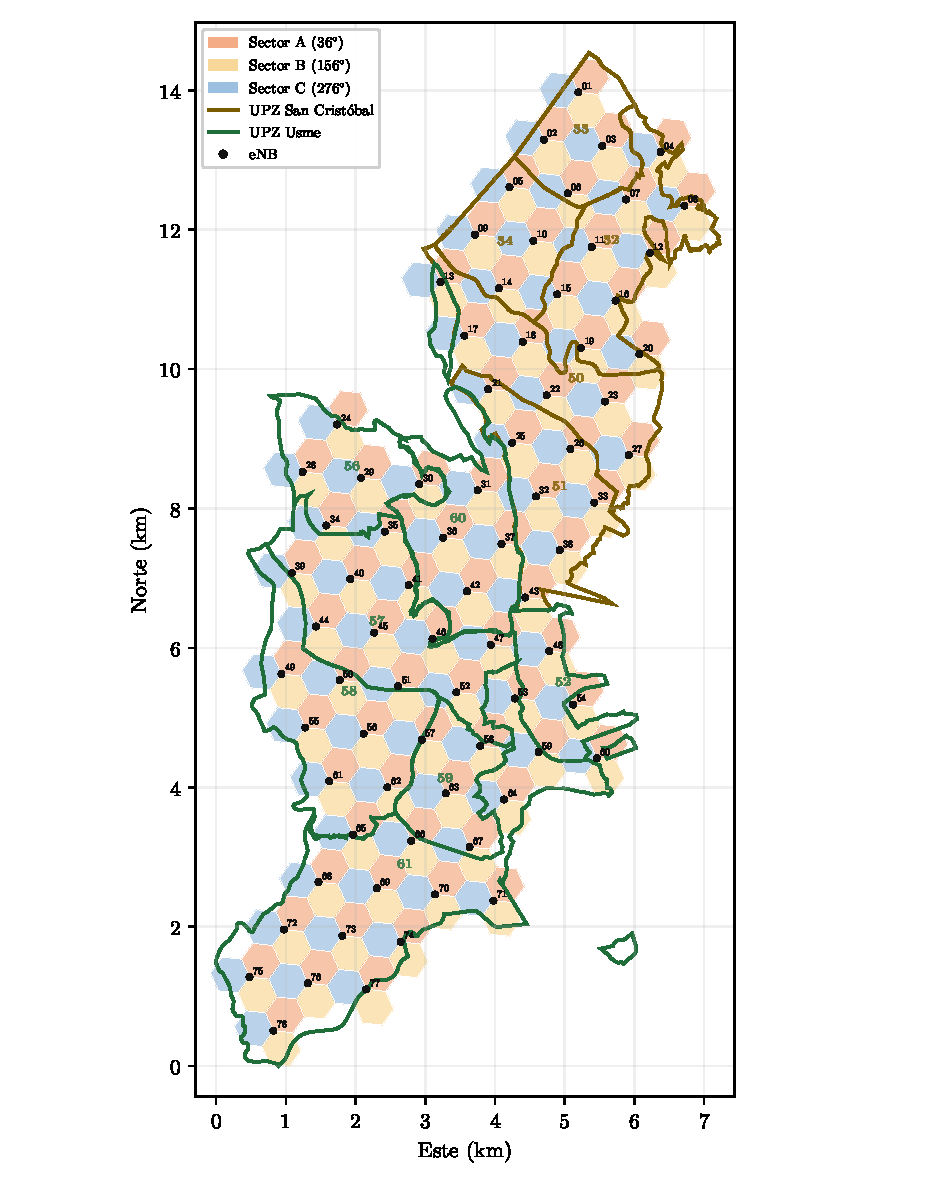
\includegraphics[width=0.78\textwidth]{mapa_enb.pdf}
\caption{Distribución de las 78 eNB y de sus sectores sobre las UPZ de San Cristóbal y Usme. Coordenadas planas MAGNA-SIRGAS Bogotá relativas a la esquina suroccidental del área. Los números en verde y ocre son los códigos de UPZ.}
\label{fig:mapa}
\end{figure}

El \SI{7.2}{\percent} sin huella hexagonal corresponde a franjas del borde irregular de las UPZ, sobre todo en los cerros de La Gloria y Los Libertadores y en el borde sur de Ciudad Usme, más un polígono aislado de Ciudad Usme al sureste. Casi todo ese borde queda dentro del radio de diseño de algún sitio vecino. Tres sitios (eNB-12, eNB-54 y eNB-60) quedan a menos de \SI{100}{m} por fuera del perímetro de las UPZ y pueden correrse hacia adentro en la etapa de adquisición de sitios. Las coordenadas de las 78 eNB están en el Anexo~\ref{anx:sitios}.

Las coordenadas son posiciones nominales de la malla. En una implementación real cada una se ajusta al predio, terraza o torre disponible más cercano (normalmente a menos de $R/4$, unos \SI{140}{m}) y se valida con mediciones en campo.

\paragraph{Archivo KML.} El archivo \texttt{Red\_LTE\_SanCristobal\_Usme\_200144723.kml} se abre en Google Earth y contiene cuatro carpetas: los límites de las 12 UPZ (ocre para San Cristóbal y verde para Usme), las 78 eNB con su ficha técnica en la descripción, los 234 sectores hexagonales con un color por sector y los círculos de radio $R=\SI{561}{m}$ (ocultos por defecto).

% ================= 9 =================
\section{Selección de equipos y características de cada eNB}

Las 78 estaciones usan la misma configuración: una unidad de banda base, tres radios remotas (una por sector) montadas junto a las antenas y tres antenas sectoriales multibanda a \SI{30}{m}.

\begin{table}[H]
\centering
\caption{Equipos seleccionados por eNB.}
\label{tab:equipos}
\small
\begin{tabularx}{\textwidth}{@{}l>{\raggedright\arraybackslash}p{3.6cm}cL@{}}
\toprule
\textbf{Elemento} & \textbf{Modelo} & \textbf{Cant.} & \textbf{Justificación} \\
\midrule
Banda base (BBU) & Ericsson Baseband 6630 & 1 & Procesa los tres sectores LTE FDD y se conecta por fibra (CPRI) a las radios. \\
Radio remota (RRU) & Ericsson Radio 4438 B2/B25 B66~\cite{ericsson} & 3 & Soporta la banda 2 del diseño y deja AWS (B66) disponible para crecer en capacidad en la Parte 2. \\
Antena sectorial & Andrew (CommScope) NHH-65B-R2B~\cite{nhh} & 3 & Seis puertos; \SIrange{698}{896}{MHz} y \SIrange{1695}{2360}{MHz} (incluye \SIrange{1850}{1990}{MHz}); haz horizontal de \SIrange{57}{71}{\degree}; inclinación variable. \\
Jumper RRU a antena & Coaxial de 1/2'' corto & 3 & Pérdida de \SI{0.5}{dB} (parámetros $H$ y $O$), con la RRU montada junto a la antena. \\
\bottomrule
\end{tabularx}
\end{table}

La hoja de datos consultada de la NHH-65B-R2B publica un rango de ganancia de \SIrange{14.9}{18.7}{dBi} entre sus bandas, sin desglose por banda. En el diseño se usó \SI{17.7}{dBi}, el valor que CommScope publica para \SIrange{1850}{1990}{MHz} en su panel HBXXX-6516DS~\cite{hbxxx} (haz de \SI{63.4}{\degree} horizontal y \SI{7.4}{\degree} vertical, inclinación eléctrica de \SIrange{2}{10}{\degree}), hoy descontinuado. Antes de la compra se debe confirmar que la ganancia en banda 2 sea de al menos \SI{17.7}{dBi}; si es menor, la MAPL de ambos enlaces baja en la misma cantidad. La potencia de \SI{40}{W} por sector es un valor de configuración; se debe verificar en la hoja de datos de la radio que esté dentro de su potencia máxima.

\begin{table}[H]
\centering
\caption{Características de diseño de cada eNB (iguales en las 78; ubicación en el Anexo~\ref{anx:sitios}).}
\label{tab:caract}
\rowcolors{2}{grisfila}{white}
\begin{tabular}{@{}ll@{}}
\toprule
\textbf{Característica} & \textbf{Valor} \\
\midrule
Tecnología & LTE FDD, banda 2, \SI{20}{MHz} (100 RB) \\
Portadora DL / UL & \SIrange{1960}{1980}{MHz} / \SIrange{1880}{1900}{MHz} \\
Sectores y azimuts & 3: A \SI{36}{\degree}, B \SI{156}{\degree}, C \SI{276}{\degree} \\
Altura de antena & \SI{30}{m} (estación tipo 3) \\
Potencia de transmisión & \SI{40}{W} (\SI{46}{dBm}) por sector \\
Ganancia de antena & \SI{17.7}{dBi} \\
EIRP por subportadora & \SI{32.41}{dBm} \\
EIRP total por sector & $46+17{,}7-0{,}5=\SI{63.2}{dBm}$ \\
Inclinación (tilt) & \SI{7}{\degree} eléctrico (RET) \\
MCS de diseño & 12 (16QAM) en DL y UL \\
Radio de celda & \SI{561}{m} \\
Área cubierta & \SI{0.613}{km^2} \\
\bottomrule
\end{tabular}
\end{table}

\paragraph{Cálculo de la inclinación.} El borde de celda se ve con un ángulo de $\arctan(30/561)=\SI{3.1}{\degree}$ bajo la horizontal. Sumando la mitad del ancho de haz vertical ($\SI{7.4}{\degree}/2=\SI{3.7}{\degree}$), el borde superior del lóbulo principal cae en el límite de la celda y se reduce la interferencia hacia los sitios vecinos: $\SI{3.1}{\degree}+\SI{3.7}{\degree}\approx\SI{7}{\degree}$. En los sitios de ladera la inclinación se corrige en campo según la diferencia de cota con el área servida.

% ================= 10 =================
\section{Conclusiones}

\begin{itemize}
  \item El enlace ascendente limita la cobertura: su MAPL es \SI{3.84}{dB} menor que la del descendente y reduce el radio de \SI{693}{m} a \SI{561}{m}. Aumentar la potencia de la eNB no reduce el número de sitios; sí lo haría mejorar la recepción en la eNB (mayor ganancia de antena, cuatro ramas de recepción o un amplificador en torre).
  \item Para las 12 UPZ urbanas (\SI{47.68}{km^2}) se requieren 78 eNB de tres sectores separadas \SI{842}{m}, 29 en San Cristóbal y 49 en Usme.
  \item El MCS 12 (16QAM) exige una SINR de \SIrange{6.8}{8.2}{dB}. Un MCS más robusto aumentaría el radio y reduciría el número de sitios a costa de la tasa en el borde de celda; ese balance se revisa en el dimensionamiento por capacidad (Parte 2).
  \item La ecuación (5) del enunciado solo da resultados coherentes si $L$ se interpreta como el término de frecuencia del modelo; con la pérdida completa a \SI{1}{km} sobrestima el radio unas 3,8 veces.
\end{itemize}

% ================= REFERENCIAS =================
\begin{thebibliography}{9}
\bibitem{enunciado} Comunicaciones Celulares, \emph{Diseño de una red celular LTE, Parte 1: Cobertura}, Universidad del Norte, 2026.
\bibitem{upz} Datos Abiertos Bogotá, \emph{Unidades de Planeamiento Zonal (UPZ), versión 06.22}. \url{https://datosabiertos.bogota.gov.co/dataset/pensionados-activos-del-foncep-por-upz}
\bibitem{sdpsc} Secretaría Distrital de Planeación, \emph{Anexo técnico, Plan de Desarrollo Local San Cristóbal 2021-2024}. \url{https://www.sdp.gov.co/sites/default/files/propuestaanexotecnico_pdl_san_cristobal.pdf}
\bibitem{sdpus} Secretaría Distrital de Planeación, \emph{Localidad de Usme}. \url{https://www.sdp.gov.co/sites/default/files/locusmevf.pdf}
\bibitem{kimovil} Kimovil, \emph{Frequency checker: Colombia}. \url{https://www.kimovil.com/es/frequency-checker/CO}
\bibitem{ericsson} Ericsson, \emph{Remote radio portfolio}. \url{https://www.ericsson.com/en/portfolio/networks/ericsson-radio-system/radio/macro/remote-radio}
\bibitem{nhh} Andrew (CommScope), \emph{NHH-65B-R2B base station antenna}. \url{https://www.everythingrf.com/products/base-station-antennas/andrew-an-amphenol-company/822-2444-nhh-65b-r2b}
\bibitem{hbxxx} CommScope, \emph{HBXXX-6516DS-VTM product specifications}. \url{https://de.commscope.com/globalassets/digizuite/262564-p360-hbxxx-6516ds-vtm-external.pdf}
\end{thebibliography}

% ================= ANEXO =================
\newpage
\appendix
\section{Ubicación de las 78 eNB}
\label{anx:sitios}

Coordenadas geográficas WGS84 en grados decimales. Todas las eNB tienen antena a \SI{30}{m} y sectores con azimuts de \SI{36}{\degree}, \SI{156}{\degree} y \SI{276}{\degree}. El símbolo $\dagger$ marca los sitios ubicados a menos de \SI{100}{m} por fuera del perímetro de las UPZ.

{\small
\rowcolors{2}{grisfila}{white}
\begin{longtable}{@{}llllr@{}}
\toprule
\textbf{eNB} & \textbf{Localidad} & \textbf{UPZ} & \textbf{Latitud} & \textbf{Longitud} \\
\midrule
\endfirsthead
\toprule
\textbf{eNB} & \textbf{Localidad} & \textbf{UPZ} & \textbf{Latitud} & \textbf{Longitud} \\
\midrule
\endhead
\bottomrule
\endfoot
eNB-01 & San Cristóbal & 33 Sosiego & 4.58421 & -74.08628 \\
eNB-02 & San Cristóbal & 33 Sosiego & 4.57805 & -74.09074 \\
eNB-03 & San Cristóbal & 33 Sosiego & 4.57725 & -74.08320 \\
eNB-04 & San Cristóbal & 32 San Blas & 4.57646 & -74.07566 \\
eNB-05 & San Cristóbal & 34 20 de Julio & 4.57189 & -74.09520 \\
eNB-06 & San Cristóbal & 33 Sosiego & 4.57110 & -74.08766 \\
eNB-07 & San Cristóbal & 32 San Blas & 4.57030 & -74.08012 \\
eNB-08 & San Cristóbal & 32 San Blas & 4.56951 & -74.07257 \\
eNB-09 & San Cristóbal & 34 20 de Julio & 4.56573 & -74.09966 \\
eNB-10 & San Cristóbal & 34 20 de Julio & 4.56494 & -74.09212 \\
eNB-11 & San Cristóbal & 32 San Blas & 4.56414 & -74.08457 \\
eNB-12$^{\dagger}$ & San Cristóbal & 32 San Blas & 4.56335 & -74.07703 \\
eNB-13 & Usme & 60 Parque Entrenubes & 4.55958 & -74.10411 \\
eNB-14 & San Cristóbal & 34 20 de Julio & 4.55878 & -74.09657 \\
eNB-15 & San Cristóbal & 32 San Blas & 4.55799 & -74.08903 \\
eNB-16 & San Cristóbal & 32 San Blas & 4.55719 & -74.08149 \\
eNB-17 & San Cristóbal & 50 La Gloria & 4.55263 & -74.10103 \\
eNB-18 & San Cristóbal & 50 La Gloria & 4.55183 & -74.09349 \\
eNB-19 & San Cristóbal & 32 San Blas & 4.55103 & -74.08595 \\
eNB-20 & San Cristóbal & 32 San Blas & 4.55024 & -74.07840 \\
eNB-21 & San Cristóbal & 51 Los Libertadores & 4.54567 & -74.09795 \\
eNB-22 & San Cristóbal & 50 La Gloria & 4.54488 & -74.09040 \\
eNB-23 & San Cristóbal & 50 La Gloria & 4.54408 & -74.08286 \\
eNB-24 & Usme & 56 Danubio & 4.54111 & -74.11749 \\
eNB-25 & San Cristóbal & 51 Los Libertadores & 4.53872 & -74.09486 \\
eNB-26 & San Cristóbal & 51 Los Libertadores & 4.53793 & -74.08732 \\
eNB-27 & San Cristóbal & 50 La Gloria & 4.53713 & -74.07978 \\
eNB-28 & Usme & 56 Danubio & 4.53495 & -74.12194 \\
eNB-29 & Usme & 56 Danubio & 4.53415 & -74.11440 \\
eNB-30 & Usme & 56 Danubio & 4.53336 & -74.10686 \\
eNB-31 & Usme & 60 Parque Entrenubes & 4.53256 & -74.09932 \\
eNB-32 & San Cristóbal & 51 Los Libertadores & 4.53177 & -74.09178 \\
eNB-33 & San Cristóbal & 51 Los Libertadores & 4.53097 & -74.08423 \\
eNB-34 & Usme & 56 Danubio & 4.52800 & -74.11886 \\
eNB-35 & Usme & 57 Gran Yomasa & 4.52720 & -74.11132 \\
eNB-36 & Usme & 60 Parque Entrenubes & 4.52641 & -74.10378 \\
eNB-37 & Usme & 60 Parque Entrenubes & 4.52561 & -74.09623 \\
eNB-38 & San Cristóbal & 51 Los Libertadores & 4.52482 & -74.08869 \\
eNB-39 & Usme & 57 Gran Yomasa & 4.52184 & -74.12332 \\
eNB-40 & Usme & 57 Gran Yomasa & 4.52104 & -74.11577 \\
eNB-41 & Usme & 57 Gran Yomasa & 4.52025 & -74.10823 \\
eNB-42 & Usme & 60 Parque Entrenubes & 4.51945 & -74.10069 \\
eNB-43 & San Cristóbal & 51 Los Libertadores & 4.51866 & -74.09315 \\
eNB-44 & Usme & 57 Gran Yomasa & 4.51489 & -74.12023 \\
eNB-45 & Usme & 57 Gran Yomasa & 4.51409 & -74.11269 \\
eNB-46 & Usme & 57 Gran Yomasa & 4.51330 & -74.10515 \\
eNB-47 & Usme & 57 Gran Yomasa & 4.51250 & -74.09761 \\
eNB-48 & Usme & 52 La Flora & 4.51171 & -74.09006 \\
eNB-49 & Usme & 58 Comuneros & 4.50873 & -74.12469 \\
eNB-50 & Usme & 58 Comuneros & 4.50794 & -74.11715 \\
eNB-51 & Usme & 57 Gran Yomasa & 4.50714 & -74.10960 \\
eNB-52 & Usme & 57 Gran Yomasa & 4.50635 & -74.10206 \\
eNB-53 & Usme & 61 Ciudad Usme & 4.50555 & -74.09452 \\
eNB-54$^{\dagger}$ & Usme & 52 La Flora & 4.50475 & -74.08698 \\
eNB-55 & Usme & 58 Comuneros & 4.50178 & -74.12160 \\
eNB-56 & Usme & 58 Comuneros & 4.50098 & -74.11406 \\
eNB-57 & Usme & 59 Alfonso López & 4.50019 & -74.10652 \\
eNB-58 & Usme & 59 Alfonso López & 4.49939 & -74.09898 \\
eNB-59 & Usme & 61 Ciudad Usme & 4.49860 & -74.09144 \\
eNB-60$^{\dagger}$ & Usme & 61 Ciudad Usme & 4.49780 & -74.08390 \\
eNB-61 & Usme & 58 Comuneros & 4.49483 & -74.11852 \\
eNB-62 & Usme & 58 Comuneros & 4.49403 & -74.11098 \\
eNB-63 & Usme & 59 Alfonso López & 4.49324 & -74.10344 \\
eNB-64 & Usme & 61 Ciudad Usme & 4.49244 & -74.09589 \\
eNB-65 & Usme & 58 Comuneros & 4.48787 & -74.11543 \\
eNB-66 & Usme & 61 Ciudad Usme & 4.48708 & -74.10789 \\
eNB-67 & Usme & 59 Alfonso López & 4.48628 & -74.10035 \\
eNB-68 & Usme & 61 Ciudad Usme & 4.48172 & -74.11989 \\
eNB-69 & Usme & 61 Ciudad Usme & 4.48092 & -74.11235 \\
eNB-70 & Usme & 61 Ciudad Usme & 4.48013 & -74.10481 \\
eNB-71 & Usme & 61 Ciudad Usme & 4.47933 & -74.09727 \\
eNB-72 & Usme & 61 Ciudad Usme & 4.47556 & -74.12435 \\
eNB-73 & Usme & 61 Ciudad Usme & 4.47476 & -74.11681 \\
eNB-74 & Usme & 61 Ciudad Usme & 4.47397 & -74.10926 \\
eNB-75 & Usme & 61 Ciudad Usme & 4.46940 & -74.12880 \\
eNB-76 & Usme & 61 Ciudad Usme & 4.46861 & -74.12126 \\
eNB-77 & Usme & 61 Ciudad Usme & 4.46781 & -74.11372 \\
eNB-78 & Usme & 61 Ciudad Usme & 4.46245 & -74.12572 \\

\end{longtable}
}

\end{document}
